\section{Implementatiediagrammen : Component- en deployment diagram}

De laatste diagrammen waar UML gebruik van maakt en waar in deze cursustekst aandacht aan besteed wordt, zijn de implementatiediagrammen. Tot nog toe hebben we ons enkel zorgen gemaakt over de analyse van de problemen en het ontwerpen van oplossingen m.b.v. objectgeoriënteerde technieken. Maar het systeem zal uiteindelijk moeten draaien op hardware waarbij het moet voldoen aan performantie-eisen en schaalbaarheid, deze dingen zijn niet-functionele eisen maar zijn evenzeer belangrijk voor het welslagen van ons project.

Vandaar de aanwezigheid van de laatste twee diagrammen, de implementatiediagrammen:

het componentdiagram toont de afhankelijkheden tussen de onderdelen van de code. 

Het deployment diagram toont de structuur van het run-time systeem: Welke onderdelen draaien waar en hoe moet de hardware geconfigureerd zijn.

\subsection{Het component diagram}

Het componentendiagram bevat :

\begin{itemize}
    \item componenten
    \item interfaces
    \item relaties
\end{itemize}

Dit diagram drukt de structuur uit van het geïmplementeerde systeem, het houdt de afhankelijkheden bij met het doel een vereenvoudiging van het onderhoud te bekomen en het hergebruik van de componenten te vergemakkelijken.

\subsection{Het component diagram: concepten}

De volgende concepten zijn van belang bij het opmaken van een component diagram:

\subsubsection{component}

\textcolor{red}{Een component is een fysiek deel van een systeem.}

Het bevindt zich in de computer, niet in de gedachten van een analist, men zou het ook "een distribueerbaar stuk van de implementatie van een systeem" kunnen noemen zo bv. een tabel, een document, een uitvoerbaar bestand...

%afbeelding nog plaatsen

\begin{center}
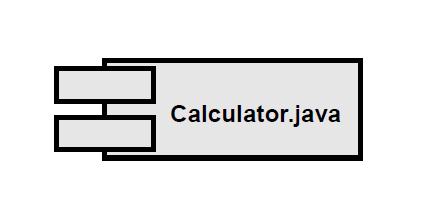
\includegraphics[width=4in]{img/component}%
\end{center}

De belangrijkste reden om met componenten te werken is de \textbf{herbruikbaarheid} die men hierdoor bereikt: men maakt een component voor een bepaald systeem en deze kan men dan hergebruiken in een ander systeem.

Door de tijd en de moeite te geven aan het modelleren van componenten, kan men zo mogelijkerwijze componenten hergebruiken.

\subsubsection{interface}

Eén van de belangrijkste principes van OO-ontwerp en programmeren is het principe van de \textbf{"inkapseling of information hiding"} dat bepaalt dat elk object voor de andere objecten en voor de buitenwereld verbergt wat dat object doet.

Maar het object moet natuurlijk wel een "gezicht" hebben naar de buitenwereld toe zodat andere objecten aan het object kunnen vragen om operaties uit te voeren.

Dit gezicht is de interface van het object.

Er zijn verschillende mogelijkheden om dit voor te stellen in het diagram:

%afbeelding nog plaatsen

\begin{center}
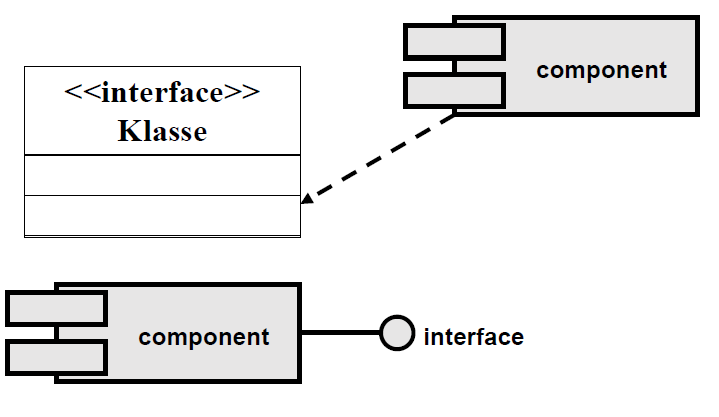
\includegraphics[width=4in]{img/interface}%
\captionof{figure}{text}
\label{labelname}%
\end{center}


